\documentclass[10pt]{article}
\usepackage[utf8]{inputenc}
\usepackage[english]{babel}
\usepackage[left=2cm, right=2cm, top=2cm, bottom=2cm]{geometry}
\usepackage{amsmath, wrapfig, pgfplots}

\pgfplotsset{compat=1.9}
\setlength\intextsep{0pt}

\begin{document}

\title{Cascaded Approximation of Gaussian Blur}
\author{Vabishchevich Nikolay}
\date{May 23, 2015}
\maketitle


\section{Basic definitions}

\begin{wrapfigure}{r}{0pt}
    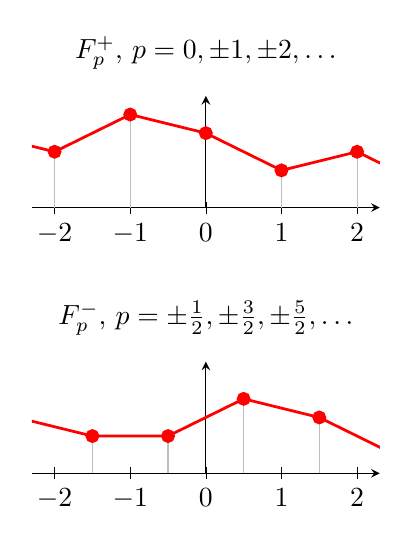
\begin{tikzpicture}
        \begin{axis} [ width = 6cm, height = 3cm, name = plot,
                title = {$F^+_p$, $p = 0, \pm1, \pm2, \ldots$},
                xmin = -2.3, xmax = 2.3, axis x line = bottom,
                xtick = {-2, ..., 2}, x tick style = { color = black },
                ymin = 0, ymax = 6, axis y line = middle, ytick = \empty ]
            \addplot [ sharp plot, mark = *, line width = 1pt, red ] coordinates
                { (-3, 4) (-2, 3) (-1, 5) (0, 4) (1, 2) (2, 3) (3, 1) };
            \addplot [ ycomb, lightgray ] coordinates
                { (-2, 3) (-1, 5) (1, 2) (2, 3) };
        \end{axis}
        \begin{axis} [ width = 6cm, height = 3cm,
                at = { (plot.below south) }, anchor = above north, yshift = -0.5cm,
                title = {$F^-_p$, $p = \pm\frac12, \pm\frac32, \pm\frac52, \ldots$},
                xmin = -2.3, xmax = 2.3, axis x line = bottom,
                xtick = {-2, ..., 2}, x tick style = { color = black },
                ymin = 0, ymax = 6, axis y line = middle, ytick = \empty ]
            \addplot [ sharp plot, mark = *, line width = 1pt, red ] coordinates
                { (-2.5, 3) (-1.5, 2) (-0.5, 2) (0.5, 4) (1.5, 3) (2.5, 1) };
            \addplot [ ycomb, lightgray ] coordinates
                { (-1.5, 2) (-0.5, 2) (0.5, 4) (1.5, 3) };
        \end{axis}
    \end{tikzpicture}
    \caption{Two types of grid placement.}
\end{wrapfigure}

In this article I'm using two different sets of grid point positions. The first one is grid point at
every integer, $F^+_k$ (I call it even and mark with ``$+$''). The second one is grid points
positioned halfway between adjacent integers, $F^-_{k+1/2}$ (I call it odd and mark with ``$-$'').
Correspondingly there are two types of convolution filters: even
\begin{equation}\label{conv+}
    R^\pm_p = \sum_{k\in Z} F^\pm_{p+k}K^+_k,
\end{equation}
and odd
\begin{equation}\label{conv-}
    R^\mp_p = \sum_{k\in Z} F^\pm_{p+k+\frac12}K^-_{k+\frac12},
\end{equation}
where $K^\pm_p$ is filter kernel. Even filter doesn't change source oddness but odd filter do (hence
the name). Therefore our target problem is to efficiently calculate approximation of
\begin{equation}
    R^\pm_p = \sum_{k\in Z} F^\pm_{p+k}G_k,
\end{equation}
where $F^\pm_p$ is the source function and $G_k$ is even Gaussian kernel,
\begin{equation}\label{gamma}
    G_k = \Gamma(\sigma^2;\, k) \equiv
        \frac1{\sqrt{2\pi\sigma^2}}\exp\left\{-\frac{k^2}{2\sigma^2}\right\},
\end{equation}
especially for large standard deviation $\sigma$.

The main tool for such task is the Fourier transform. I'm using it in the following form:
\begin{align}
    F^+(\varphi) &= \sum_{k\in Z} F^+_k e^{ik\varphi},\\
    F^-(\varphi) &= \sum_{k\in Z} F^-_{k+\frac12} e^{i(k+\frac12)\varphi},
\end{align}
\begin{equation}
    F^\pm_p = \frac1{2\pi}\int_{-\pi}^\pi F^\pm(\varphi)e^{-ip\varphi}d\varphi.
\end{equation}
As usual, Fourier transform of real function satisfies
\begin{equation}
    F^\pm(-\varphi) = F^{\pm*}(\varphi).
\end{equation}
Also due to discreteness holds the following (another source of the even/odd name):
\begin{equation}
    F^\pm(\varphi+2\pi) = \pm F^\pm(\varphi).
\end{equation}
For symmetric (relative to 0) functions its Fourier amplitude is strictly real.

For convolutional filter with even kernel $K^+_p$ (\ref{conv+}) holds
\begin{equation}
    R^\pm(\varphi) = F^\pm(\varphi)K^{+*}(\varphi).
\end{equation}
In case of odd kernel $K^-_p$ (\ref{conv-}),
\begin{equation}
    R^\mp(\varphi) = F^\pm(\varphi)K^{-*}(\varphi).
\end{equation}
For symmetric filters it's possible to drop conjugation sign in these equations.

In the following I'll need transforms of basic binomial filters. That's well known sequence of
filters, kernels of which from the beginning of the sequence look like
\begin{align}
    \label{B1} B^1 &= [1, 1] / 2,\\
    \label{B2} B^2 &= [1, 2, 1] / 4,\\
    \label{B3} B^3 &= [1, 3, 3, 1] / 8,\\
    \label{B4} B^4 &= [1, 4, 6, 4, 1] / 16,\\
    \label{B5} B^5 &= [1, 5, 10, 10, 5, 1] / 32,\\
    \label{B6} B^6 &= [1, 6, 15, 20, 15, 6, 1] / 64,\\
                   &\cdots\nonumber
\end{align}
Filters from the sequence at even index is even and of odd index is odd. Also it's easy to see that
effect from high order filter $B^n$ is the same as from the first filter $B^1$ (or simply $B$)
applied $n$ times. Hence its Fourier transform is
\begin{equation}
    B^n(\varphi) = \cos^n\frac\varphi2.
\end{equation}

\pgfplotsset{spectrum/.style = {
    width = 6cm, height = 6cm, domain = -1:1, samples = 256,
    xtick = {-1, 0, 1}, xticklabels = {$-\pi$, $0$, $\pi$}, minor x tick num = 1,
    xmin = -1, xmax = 1, xminorgrids = true, xmajorgrids = true,
    ymin = 0, ymax = 1, yminorgrids = true, ymajorgrids = true,
}}
\begin{wrapfigure}{r}{0pt}
    \begin{tikzpicture}
        \begin{axis} [ spectrum, title = $G(\varphi)$ ]
            \addplot [ sharp plot, line width = 1pt, red ] gnuplot {
                exp(-8*(x*pi)^2)
            };
        \end{axis}
    \end{tikzpicture}
    \caption{Gaussian spectrum (\ref{gauss}) for $\sigma^2 = 16$.}
\end{wrapfigure}

Going back to our Gaussian filter (\ref{gamma}), its Fourier transform is another Gaussian function
\begin{equation}\label{gauss}
    G(\varphi) \approx \exp\left\{-\frac{\sigma^2\varphi^2}2\right\}.
\end{equation}
That function has two different regions. The first is almost zero at high frequency and the second
is bell-like shape at low frequency. Correspondingly the task of approximation can be divided into
two subtasks described in the following sections.


\section{Zeroing high frequency}

The only way to avoid large filter kernels in approximation of Gaussian blur with large radius is to
somehow reduce resolution before filtering. That can be done through successive steps of shrinking
by factor of two, then applying main filter and then expanding twofold the same number of steps.
Central main filter will be examined in the next section and this section concentrates on scaling.

The basic operation for such task is dropping every second point from grid. For even function
$F^+_k$ there are two ways to do so. First is to keep only even points (I call it operator
$\hat S_+$)
\begin{equation}
    R^+_k = F^+_{2k}.
\end{equation}
Second is to keep odd (operator $\hat S_-$)
\begin{equation}
    R^-_{k+\frac12} = F^+_{2k+1}.
\end{equation}
Its Fourier transforms look like
\begin{equation}\label{S}
    R^\pm(\varphi) =
        \frac12 \left[F^+\left(\frac\varphi2\right) \pm F^+\left(\pi+\frac\varphi2\right)\right].
\end{equation}
Complementary operation for expanding is inserting zeroes between each neighbour pair of values.
Similarly there are two versions, even (operator $\hat S^\dagger_+$)
\begin{equation}
    R^+_n = \left\{
        \begin{array}{ll}
            F^+_k,& n = 2k;\\
            0,& n = 2k + 1.
        \end{array}
    \right.
\end{equation}
and odd (operator $\hat S^\dagger_-$ correspondingly)
\begin{equation}
    R^+_n = \left\{
        \begin{array}{ll}
            0,& n = 2k;\\
            F^-_{k+\frac12},& n = 2k + 1.
        \end{array}
    \right.
\end{equation}
Fourier transform of the result of that operation is quite direct
\begin{equation}
    R^+(\varphi) = F^\pm(2\varphi).
\end{equation}

\begin{figure}[t]
    \centering
    \begin{tikzpicture}
        \begin{axis} [ spectrum, name = plot1, title = $F^+$ ]
            \addplot [ sharp plot, line width = 1pt, domain = -1:-0.5, blue] gnuplot {
                0.8 * exp(-(x*pi)^2) + 0.4 * exp(-8*((abs(x)-1)*pi)^2)
            };
            \addplot [ sharp plot, line width = 1pt, domain = -0.5:0.5, green] gnuplot {
                0.8 * exp(-(x*pi)^2) + 0.4 * exp(-8*((abs(x)-1)*pi)^2)
            };
            \addplot [ sharp plot, line width = 1pt, domain = 0.5:1, blue] gnuplot {
                0.8 * exp(-(x*pi)^2) + 0.4 * exp(-8*((abs(x)-1)*pi)^2)
            };
        \end{axis}
    \end{tikzpicture}
    \begin{tikzpicture}
        \begin{axis} [ spectrum, name = plot2, title = $\hat S_+F^+$,
                at = { (plot1.right of east) }, anchor = left of west, xshift = 0.5cm ]
            \addplot [ sharp plot, line width = 1pt, green ] gnuplot {
                0.4 * exp(-(x*pi/2)^2)
            };
            \addplot [ sharp plot, line width = 1pt, blue ] gnuplot {
                0.4 * exp(-((abs(x/2)-1)*pi)^2) + 0.2 * exp(-8*(x*pi/2)^2)
            };
            \addplot [ sharp plot, line width = 1pt, red ] gnuplot {
                0.4 * exp(-(x*pi/2)^2) +
                0.4 * exp(-((abs(x/2)-1)*pi)^2) + 0.2 * exp(-8*(x*pi/2)^2)
            };
        \end{axis}
    \end{tikzpicture}
    \begin{tikzpicture}
        \begin{axis} [ spectrum, name = plot3, title = $\hat S^\dagger_+\hat S_+F^+$,
                at = { (plot2.right of east) }, anchor = left of west, xshift = 0.5cm ]
            \addplot [ sharp plot, line width = 1pt, red ] gnuplot {
                0.4 * exp(-(x*pi)^2) + 0.2 * exp(-8*((abs(x)-1)*pi)^2) +
                0.4 * exp(-((abs(x)-1)*pi)^2) + 0.2 * exp(-8*(x*pi)^2)
            };
        \end{axis}
    \end{tikzpicture}
    \caption{Spectrum of the source function $F^+(\varphi)$ after successive application of basic
        shrink $\hat S_+$ and expand $\hat S^\dagger_+$ operators.}
\end{figure}

Basic shrink/expand operations is not much useful as is due to several problems. Shrink operator
$\hat S_\pm$ isn't conservative ($R(\varphi)\neq F(\varphi)$) and high-frequency part contaminate
low-frequency. Expand operator $\hat S^\dagger_\pm$ duplicates low-frequency part into
high-frequency instead of zeroing it. To solve these problems I apply additional convolutional
filters before shrinking and after expanding. More particularly, the full shrink operator is
\begin{equation}\label{P}
    \hat P = 2\hat S\hat K_{\text{in}},
\end{equation}
where $2$ denotes multiplication by $2$ to get rid of $\frac12$ factor from (\ref{S}). The filter
kernel $K_{\text{in}}(\varphi)$ should be exactly zero at $\varphi = \pm\pi$ for conservation and be
quite small in all high half of the spectrum. Similarly, the full expand operator is
\begin{equation}\label{Q}
    \hat Q = \hat K_{\text{out}}\hat S^\dagger,
\end{equation}
where the filter kernel $K_{\text{out}}(\varphi)$ should be small at high-frequency.

Consider the following process: apply the shrink operator $\hat P$, then some convolutional filter
$\hat T$, than expand operator $\hat Q$. Fourier transform of the result can be easily calculated
through
\begin{align}
    (\hat K_{\text{in}}F)(\varphi) &= K_{\text{in}}(\varphi)F(\varphi),\\
    (\hat PF)(\varphi) &=
        K_{\text{in}}\left(\frac\varphi2\right)F\left(\frac\varphi2\right) \pm
        K_{\text{in}}\left(\pi+\frac\varphi2\right)F\left(\pi+\frac\varphi2\right),\\
    (\hat T\hat PF)(\varphi) &= \left[
        K_{\text{in}}\left(\frac\varphi2\right)F\left(\frac\varphi2\right) \pm
        K_{\text{in}}\left(\pi+\frac\varphi2\right)F\left(\pi+\frac\varphi2\right)
        \right]T(\varphi),\\
    (\hat S^\dagger\hat T\hat PF)(\varphi) &= \left[K_{\text{in}}(\varphi)F(\varphi) \pm
        K_{\text{in}}(\pi+\varphi)F(\pi+\varphi)\right]T(2\varphi),\\
    R(\varphi) = (\hat Q\hat T\hat PF)(\varphi) &= \left[K_{\text{in}}(\varphi)F(\varphi) \pm
        K_{\text{in}}(\pi+\varphi)F(\pi+\varphi)\right]T(2\varphi)K_{\text{out}}(\varphi).
\end{align}
It's easy to see that there are two components in the result, good
\begin{equation}
    R_{\text{good}}(\varphi) =
        K_{\text{in}}(\varphi)T(2\varphi)K_{\text{out}}(\varphi)\cdot F(\varphi)
\end{equation}
with effect of convolutional filter with kernel
$K_{\text{in}}(\varphi)T(2\varphi)K_{\text{out}}(\varphi)$, and bad
\begin{equation}
    R_{\text{bad}}(\varphi) =
        K_{\text{in}}(\pi+\varphi)T(2\varphi)K_{\text{out}}(\varphi)\cdot F(\pi+\varphi),
\end{equation}
which corresponds to frequency contamination.

Previous equations don't have any ``$+$'' or ``$-$'' signs due to many possible even/odd
combinations. In computer graphics grid points usually correspond to centers of pixel squares so I
limit myself mainly to odd intermediate functions. As input to elementary shrink operator $\hat S$
should be even function, filter $\hat K_{\text{in}}$ should be odd to compensate oddness of the
input to operator $\hat P$. Similarly, filter $\hat K_{\text{out}}$ should be odd due to even output
of $\hat S^\dagger$. Also $\hat P$ and $\hat Q$ should use odd versions of the elementary
shrink/expand operator. Therefore the accurate version of equations (\ref{P}) and (\ref{Q}) look
like
\begin{equation}
    \hat P = 2\hat S_-\hat K^-_{\text{in}},\quad
    \hat Q = \hat K^-_{\text{out}}\hat S^\dagger_-.
\end{equation}

\begin{figure}[t]
    \centering
    \begin{tikzpicture}
        \begin{axis} [ spectrum, name = plot1,
                title = { $\hat K_{\text{in}} = \hat K_{\text{out}} = \hat B^1$ } ]
            \addplot [ sharp plot, line width = 1pt, red] gnuplot {
                cos(x*pi/2)^(2*1)
            };
            \addplot [ sharp plot, line width = 1pt, green] gnuplot {
                abs(cos(x*pi/2) * sin(x*pi/2))^1
            };
        \end{axis}
    \end{tikzpicture}
    \begin{tikzpicture}
        \begin{axis} [ spectrum, name = plot2,
                title = { $\hat K_{\text{in}} = \hat K_{\text{out}} = \hat B^3$ },
                at = { (plot1.right of east) }, anchor = left of west, xshift = 0.5cm ]
            \addplot [ sharp plot, line width = 1pt, red] gnuplot {
                cos(x*pi/2)^(2*3)
            };
            \addplot [ sharp plot, line width = 1pt, green] gnuplot {
                abs(cos(x*pi/2) * sin(x*pi/2))^3
            };
        \end{axis}
    \end{tikzpicture}
    \begin{tikzpicture}
        \begin{axis} [ spectrum, name = plot3,
                title = { $\hat K_{\text{in}} = \hat K_{\text{out}} = \hat B^5$ },
                at = { (plot2.right of east) }, anchor = left of west, xshift = 0.5cm ]
            \addplot [ sharp plot, line width = 1pt, red] gnuplot {
                cos(x*pi/2)^(2*5)
            };
            \addplot [ sharp plot, line width = 1pt, green] gnuplot {
                abs(cos(x*pi/2) * sin(x*pi/2))^5
            };
        \end{axis}
    \end{tikzpicture}
    \caption{Total effect and absolute value of frequency contamination for $\hat Q\hat P$.}
    \label{scale}
\end{figure}

\begin{figure}[t]
    \centering
    \begin{tikzpicture}
        \begin{axis} [ spectrum, name = plot1,
                title = { $\hat K_{\text{in}} = \hat K_{\text{out}} = \hat B^1$ } ]
            \addplot [ sharp plot, line width = 1pt, red] gnuplot {
                (cos(x*pi/2) * cos(x*pi))^(2*1)
            };
        \end{axis}
    \end{tikzpicture}
    \begin{tikzpicture}
        \begin{axis} [ spectrum, name = plot2,
                title = { $\hat K_{\text{in}} = \hat K_{\text{out}} = \hat B^3$ },
                at = { (plot1.right of east) }, anchor = left of west, xshift = 0.5cm ]
            \addplot [ sharp plot, line width = 1pt, red] gnuplot {
                (cos(x*pi/2) * cos(x*pi))^(2*3)
            };
        \end{axis}
    \end{tikzpicture}
    \begin{tikzpicture}
        \begin{axis} [ spectrum, name = plot3,
                title = { $\hat K_{\text{in}} = \hat K_{\text{out}} = \hat B^5$ },
                at = { (plot2.right of east) }, anchor = left of west, xshift = 0.5cm ]
            \addplot [ sharp plot, line width = 1pt, red] gnuplot {
                (cos(x*pi/2) * cos(x*pi))^(2*5)
            };
        \end{axis}
    \end{tikzpicture}
    \caption{Effect of double stage shrinking/expanding operation $\hat Q^2\hat P^2$.}
    \label{scale2}
\end{figure}

Now it's time to choose $\hat K_{\text{in/out}}$. One of the possible variants is odd binomial
filters (\ref{B1}), (\ref{B3}), (\ref{B5}), etc. Also I use the same filter for both $\hat
K_{\text{in}}$ and $\hat K_{\text{out}}$ for simplicity and to move error into the range of minimal
values of bell-like $T(\varphi)$. Given
\begin{equation}
    K_{\text{in}}(\varphi) = K_{\text{out}}(\varphi) = B^n(\varphi) = \cos^n\frac\varphi2,
\end{equation}
we have
\begin{align}
    R_{\text{good}}(\varphi) &= \cos^{2n}\frac\varphi2 \cdot T(2\varphi)F(\varphi),\\
    R_{\text{bad}}(\varphi) &= \cos^n\frac\varphi2\sin^n\frac\varphi2 \cdot T(2\varphi)F(\pi+\varphi).
\end{align}
Fig.~\ref{scale} shows factors of $R_{\text{good}}$ and $R_{\text{bad}}$ independent from $F$ and
$T$ for different choice of odd $n$. Fig.~\ref{scale2} shows total effect (effective kernel) of
two-stage rescaling. As we can see, $\hat B^1$ is terribly bad: up to 50\% crosstalk, large
high-frequency half, bad stackability. $\hat B^3$ is much better: maximal crosstalk is 12.5\% with
$R_{\text{bad}}(\varphi) \propto \varphi^3$ near zero, no problem with stackability. While that's
quite good it's not enough for desired integral error to be less than 0.5\% so I ended with $\hat
B^5$. Its max crosstalk is about 3.1\% with $R_{\text{bad}}(\varphi) \propto \varphi^5$ around zero,
bell-shaped $T(\varphi)$ fall into that near-zero region and integral error can be quite small.
Therefore final versions of rescale operators is
\begin{equation}
    \hat P = 2\hat S_-\hat B^5,\quad
    \hat Q = \hat B^5\hat S^\dagger_-.
\end{equation}


\section{Main low-frequency filter}

For last task of approximating central Gaussian shape I've decided to use generic 9-tap filter as
the main workhorse. Under that name I imply even symmetric conservative convolutional filter of the
following form
\begin{equation}\label{main}
    K_k = \left\{
        \begin{array}{ll}
            1 - 2\sum_{i=1}^4 C_i,& k = 0;\\
            C_i,& k = m_i;\\
            0,& \text{otherwise};
        \end{array}
    \right.
\end{equation}
where $m_i$, $i=1, 2, 3, 4$, are sampling positions ($0 < m_1 < m_2 < m_3 < m_4$) and $C_i$ are
coefficients. Fourier transform of this filter kernel is
\begin{equation}
    K(\varphi) = 1 - \sum_{i=1}^4 C_i[2 - 2\cos(m_i\varphi)].
\end{equation}
Further research shows that this filter isn't enough as central filter so I combine it with
additional stage of even binomial filter $\hat B^{2l}$ ($B^0$ mean ``do nothing''). Therefore
complete approximation of Gaussian blur take the form of
\begin{equation}
    \hat G_{\text{apx}} = \hat Q^n\hat K\hat B^{2l}\hat P^n.
\end{equation}
Disregarding frequency crosstalk, diagonal part of that operator in Fourier space is
\begin{equation}
    G_{\text{apx}}(\varphi) = \left\{1 - \sum_{i=1}^4 C_i[2 - 2\cos(2^nm_i\varphi)]\right\}
        \cos^{2l}(2^{n-1}\varphi) \prod_{k=0}^{n-1} \cos^{10}(2^{k-1}\varphi).
\end{equation}
Outside of the region $[-\pi/2^n, \pi/2^n]$ that should be already near zero, so we focus only on
center
\begin{equation}
    G_{\text{apx}}\left(\frac\varphi{2^n}\right) =
        \left\{1 - \sum_{i=1}^4 C_i[2 - 2\cos(m_i\varphi)]\right\}
        \cos^{2l}\frac\varphi2 \prod_{k=1}^n \cos^{10}\frac\varphi{2^{k+1}},
\end{equation}
where that expression should be near
\begin{equation}
    G\left(\frac\varphi{2^n}\right) = \exp\left\{-\frac{\sigma^2\varphi^2}{2\cdot4^n}\right\}.
\end{equation}

One of the possible ways to find good kernel coefficients $C_i$ is to solve least squares problem.
Denote
\begin{equation}
    p(\varphi) \equiv \cos^{2l}\frac\varphi2 \prod_{k=1}^n \cos^{10}\frac\varphi{2^{k+1}}
\end{equation}
and
\begin{equation}
    g(\varphi) \equiv \exp\left\{-\frac{\sigma^2\varphi^2}{2\cdot4^n}\right\},
\end{equation}
then the problem is to minimize
\begin{equation*}
    \lambda = \int_{-\pi}^\pi \left[G\left(\frac\varphi{2^n}\right) -
        G_{\text{apx}}\left(\frac\varphi{2^n}\right)\right]^2 w(\varphi) d\varphi =
\end{equation*}
\begin{equation*}
    \int_{-\pi}^\pi \left[g(\varphi) -
        \left\{1 - \sum_{i=1}^4 C_i[2 - 2\cos(m_i\varphi)]\right\}p(\varphi)\right]^2
        w(\varphi) d\varphi =
\end{equation*}
\begin{equation}\label{lambda}
    \int_{-\pi}^\pi \left[g(\varphi) - p(\varphi) +
        p(\varphi)\sum_{i=1}^4 C_i[2 - 2\cos(m_i\varphi)]\right]^2 w(\varphi) d\varphi,
\end{equation}
where $w(\varphi) \approx 1$ is additional weight. As usual, calculating partial derivatives
\begin{equation*}
    0 = \frac12\frac{\partial\lambda}{\partial C_k} =
    \int_{-\pi}^\pi \left[g(\varphi) - p(\varphi) +
        p(\varphi)\sum_{i=1}^4 C_i[2 - 2\cos(m_i\varphi)]\right]
        p(\varphi)w(\varphi)[2 - 2\cos(m_k\varphi)] d\varphi =
\end{equation*}
\begin{equation}
    \int_{-\pi}^\pi [g(\varphi) - p(\varphi)]p(\varphi)w(\varphi)[2 - 2\cos(m_k\varphi)] d\varphi +
    \sum_{i=1}^4 C_i\int_{-\pi}^\pi p^2(\varphi)w(\varphi)
        [2 - 2\cos(m_i\varphi)][2 - 2\cos(m_k\varphi)] d\varphi.
\end{equation}
After defining
\begin{equation}
    U_k \equiv \frac1{2\pi}\int_{-\pi}^\pi p^2(\varphi)w(\varphi)e^{-ip\varphi}d\varphi
\end{equation}
and
\begin{equation}
    V_k \equiv \frac1{2\pi}\int_{-\pi}^\pi g(\varphi)p(\varphi)w(\varphi)e^{-ip\varphi}d\varphi
\end{equation}
we can get
\begin{equation}
    0 = \frac1{4\pi}\frac{\partial\lambda}{\partial C_k} = 2[V_0 - V_{m_k} - U_0 + U_{m_k}] +
        2\sum_{i=1}^4 C_i[2U_0 - 2U_{m_i} - 2U_{m_k} + U_{m_i+m_k} + U_{|m_i-m_k|}].
\end{equation}
Resulting symmetric system of four linear equations
\begin{equation}
    \sum_{i=1}^4 C_i[2U_0 - 2U_{m_i} - 2U_{m_k} + U_{m_i+m_k} + U_{|m_i-m_k|}] =
        U_0 - U_{m_k} - V_0 + V_{m_k},
\end{equation}
can be solved through standard methods of linear algebra.

The real problem here is to efficiently calculate $U_k$ and $V_k$. One method is to use crude
approximation
\begin{equation}
    p(\varphi) \approx \exp\left\{-\frac{\alpha\varphi^2}2\right\},
\end{equation}
where
\begin{equation}\label{alpha}
    \alpha = \frac l2 + \frac56(1 - 4^{-n}).
\end{equation}
In that case
\begin{equation}
    U_k \approx \frac1{2\pi}\int_{-\pi}^\pi
        \exp\left\{-\alpha\varphi^2\right\}e^{-ip\varphi}d\varphi \approx \Gamma(2\alpha;\, k),
\end{equation}
\begin{equation}\label{V-gauss}
    V_k \approx \frac1{2\pi}\int_{-\pi}^\pi
        \exp\left\{-\left[\frac{\sigma^2}{4^n} + \alpha\right]\frac{\varphi^2}2\right\}
        e^{-ip\varphi}d\varphi \approx \Gamma(\sigma^24^{-n} + \alpha;\, k),
\end{equation}
where $\Gamma$ is normalized Gaussian function defined in (\ref{gamma}).

Much better method is to choose $w(\varphi)$ such that
\begin{equation}
    p(\varphi)w(\varphi) = \exp\left\{-\frac{\alpha\varphi^2}2\right\}
\end{equation}
holds exactly. In that case (\ref{V-gauss}) holds exactly too and for $U_k$ we
have
\begin{equation}
    U_k = \frac1{2\pi}\int_{-\pi}^\pi \exp\left\{-\frac{\alpha\varphi^2}2\right\}
        p(\varphi)e^{-ip\varphi}d\varphi =
    \frac1{2\pi}\int_{-\pi}^\pi \exp\left\{-\frac{\alpha\varphi^2}2\right\}
        B^{2l}(\varphi)D(\varphi)e^{-ip\varphi}d\varphi,
\end{equation}
where $D$ is effective rescale filter kernel with
\begin{equation}
    D(\varphi) \equiv \prod_{k=1}^n \cos^{10}\frac\varphi{2^{k+1}}.
\end{equation}
Therefore $U_k$ can be calculated in the following way: construct Gaussian function
$\Gamma(\alpha;\, k)$, then apply filter $\hat D$, than apply binomial filter of order $2l$.
Alternatively that can be written in operator notation as
\begin{equation}
    \hat U = \hat B^{2l}\hat D\,\hat\Gamma(\alpha;\, \cdot).
\end{equation}

And the third method is to use $w(\varphi) = 1$ and calculate all precisely. In that case
\begin{equation}
    U_k = \frac1{2\pi}\int_{-\pi}^\pi B^{4l}(\varphi)D^2(\varphi)e^{-ip\varphi}d\varphi,
\end{equation}
\begin{equation}
    V_k = \frac1{2\pi}\int_{-\pi}^\pi
        \exp\left\{-\frac{\sigma^2\varphi^2}{2\cdot4^n}\right\}
        B^{2l}(\varphi)D(\varphi)e^{-ip\varphi}d\varphi,
\end{equation}
or alternatively
\begin{align}
    \hat U &= \hat B^{4l}\hat D^2,\\
    \hat V &= \hat B^{2l}\hat D\,\hat\Gamma(\sigma^24^{-n};\, \cdot).
\end{align}

\begin{figure}[t]
    \centering
    \begin{tikzpicture}
        \begin{axis} [ spectrum, width = 8cm, height = 8cm,
                name = plot1, title = { $D(\varphi)$, $n = 1$ } ]
            \addplot [ sharp plot, line width = 1pt, blue ] gnuplot {
                cos(x*pi/4)^10
            };
            \addplot [ sharp plot, line width = 1pt, red ] gnuplot {
                (381024 + 181440 * 2*cos(x*pi) + 15120 * 2*cos(2*x*pi)) / 774144
            };
        \end{axis}
        \begin{axis} [ spectrum, width = 8cm, height = 8cm,
                name = plot2, title = { $D(\varphi)$, $n = 2$ },
                at = { (plot1.right of east) }, anchor = left of west, xshift = 0.5cm ]
            \addplot [ sharp plot, line width = 1pt, blue ] gnuplot {
                cos(x*pi/4)^10 * cos(x*pi/8)^10
            };
            \addplot [ sharp plot, line width = 1pt, red ] gnuplot {
                (21981456 + 11993940 * 2*cos(x*pi) +
                1746360 * 2*cos(2*x*pi) + 41580 * 2*cos(3*x*pi)) / 49545216
            };
        \end{axis}
    \end{tikzpicture}
    \caption{Approximation of rescale kernel $D$ (exact curve showed as blue).}
    \label{D}
\end{figure}

Third method is usually slightly better than second and much better then first, but precise methods
require good approximation of effective rescale filter $D$. Experiments shows that tight 7-tap
approximation
\begin{equation}
    D(\varphi) \approx D_0 + 2\sum_{k=1}^3 D_k\cos(k\varphi)
\end{equation}
is quite good. Coefficients here should be chosen in such a way that equation is exact up to 6
term of Taylor series around $\varphi = 0$. Corresponding problem can be solved analytically
and give the following results
\newcommand\0{\phantom{0}}
\begin{align}
    D_0 &= (   5204 +   2520\cdot4^{-n} +   1092\cdot16^{-n} +   3280\cdot64^{-n}) / 12096,\\
    D_1 &= (   2943 - \0 210\cdot4^{-n} - \0 273\cdot16^{-n} -   2460\cdot64^{-n}) / 12096,\\
    D_2 &= (\0  486 - \0 924\cdot4^{-n} - \0 546\cdot16^{-n} + \0 984\cdot64^{-n}) / 12096,\\
    D_3 &= (\0\0 17 - \0 126\cdot4^{-n} + \0 273\cdot16^{-n} - \0 164\cdot64^{-n}) / 12096.
\end{align}
Fig.~\ref{D} shows that such approximation noticeably differ from exact curve only at region near
$\varphi = \pm\pi$ where the target Gaussian is near zero anyway. Accurate approximation of
effective rescale filter kernel concludes calculation of the main filter coefficients, and in the
following section I'll study the task of choosing remaining parameters $n$, $l$ and $m_i$.


\section{Error estimation and mode selection}

Value selection for integer parameters is quite straightforward: try different parameter sets,
estimate error and choose best in some sense. Key process here is calculation of that estimate. One
of the possible ways is to use mean square error (\ref{lambda}) from previous section but I use
more accurate method.

Combined effect of all stages of Gaussian blur approximation can be written in generic form
\begin{equation}
    R_i = \sum_{j\in Z} K_{ij}F_j,
\end{equation}
where
\begin{equation}
    K_{ij} \approx G_{i-j} = \Gamma(\sigma^2;\, i - j) =
        \frac1{\sqrt{2\pi\sigma^2}}\exp\left\{-\frac{(i - j)^2}{2\sigma^2}\right\}.
\end{equation}
Assuming that filter doesn't distort constant function (if $F_i = c$ then $R_i = c$) or
alternatively
\begin{equation}
    \sum_{j\in Z} K_{ij} = 1,
\end{equation}
and source values lie between $0$ and $1$,
\begin{equation}
    0 \le F_i \le 1,
\end{equation}
we can calculate exact upper bound of error $E^{\max}_i = \sup_F |E_i|$, where
\begin{equation}\label{E}
    E_i = \sum_{j\in Z} [K_{ij} - G_{i-j}]F_j.
\end{equation}
Due to zero error in case of zero source function
\begin{equation}
    E^{\max}_i = \sup_F |E_i| = \max\{-\inf_F E_i,\; \sup_F E_i\}.
\end{equation}
To calculate maximum positive and negative error one can choose $F_j$ in such a way that sum from
(\ref{E}) reduces to sum of only positive or negative terms,
\begin{align}
    \inf_F E_i &= \sum_{j\in Z, K_{ij} < G_{i-j}} [K_{ij} - G_{i-j}],\\
    \sup_F E_i &= \sum_{j\in Z, K_{ij} > G_{i-j}} [K_{ij} - G_{i-j}].
\end{align}
It's easy to see that
\begin{align}
    \sup_F E_i + \inf_F E_i &= \sum_{j\in Z} [K_{ij} - G_{i-j}] = 1 - 1 = 0,\\
    \sup_F E_i - \inf_F E_i &= \sum_{j\in Z} |K_{ij} - G_{i-j}|,
\end{align}
and
\begin{equation}
    E^{\max}_i = \max\{-\inf_F E_i,\; \sup_F E_i\} = \sup_F E_i =
        \frac12\sum_{j\in Z} |K_{ij} - G_{i-j}|.
\end{equation}
That's the final form of error estimation I'll use later.

Considerable experimentation shows that there is 3 types of main filter pattern worth exploring.
Those are
\begin{align}
    m^\alpha_i &= \{1, 2, 3, 4\},\\
    m^\beta_i  &= \{1, 2, 3, 5\},\\
    m^\gamma_i &= \{1, 2, 4, 6\}.
\end{align}
I call it ``1234'', ``1235'' and ``1246'' respectively. Also I consider the following types of
binomial auxiliary stage: $l = 0$ (do nothing), $l = 1$ (\ref{B2}), $l = 2$ (\ref{B4}) and $l = 3$
(\ref{B6}). Specific values of error bound is depicted at fig.~\ref{modes} for different
supplementary and main filter pairs. We can see that uniform precision is limited by error of 0.12\%
for $\sigma^2 \approx 6.693$. Taking that value into consideration and also the fact that use of
lower values of $l$ is preferable (better performance) I ended up with the following strategy.
\begin{itemize}
    \item If $\sigma^2 < 1.9$ then use single filter ``1234'' in direct mode---with coefficients
        from (\ref{gamma}). Don't perform any rescaling ($n = 0$) and don't use any additional
        filters ($l = 0$).
    \item Otherwise if $1.9 \le \sigma^2 < 6.693$ then skip rescaling ($n = 0$) but use nontrivial
        auxiliary filter.
        \begin{itemize}
            \item For $1.9 \le \sigma^2 < 2.8$   use filter ``1234'' with $\hat B^2$ ($l = 1$).
            \item For $2.8 \le \sigma^2 < 4.4$   use filter ``1235'' with $\hat B^4$ ($l = 2$).
            \item For $4.4 \le \sigma^2 < 6.693$ use filter ``1246'' with $\hat B^6$ ($l = 3$).
        \end{itemize}
    \item Else ($\sigma^2 \ge 6.693$) calculate number of shrinking/expanding stages as
        \begin{equation}
            n = 2 + \left\lfloor\log_4\frac{\sigma^2 + 0.7}{26.5}\right\rfloor,
        \end{equation}
        and scaled dispersion
        \begin{equation}
            \tilde\sigma^2 = \sigma^2\cdot4^{-n}.
        \end{equation}
        \begin{itemize}
            \item If $\tilde\sigma^2 < 3.15 - 1.5\cdot4^{-n}$ then
                use single filter ``1234'' ($l = 0$).
            \item Else if $\tilde\sigma^2 < 5.3 - 5.2\cdot4^{-n}$ then
                use filter ``1235'' with $\hat B^2$ ($l = 1$).
            \item Otherwise use filter ``1246'' with $\hat B^4$ ($l = 2$).
        \end{itemize}
\end{itemize}
There is a possibility that such strategy can result in negative main filter coefficients $C_i$
(\ref{main}).  It's undesirable due to probability of overflow of initial $[0, 1]$ range. So I
truncate such coefficients to zero. That increases error in certain areas but do not degrades global
precision. The final error bound achieved by the full algorithm is displayed in fig.~\ref{error}.

\pgfplotstableread{error.table}\errortable
\begin{figure}[t]
    \centering
    \begin{tikzpicture}
        \begin{semilogxaxis} [ title = $E_{\max}(\sigma^2)$,
                width = 18cm, height = 6cm, scaled ticks = false,
                xmin = 1, xmax = 10000, xminorgrids = true, xmajorgrids = true,
                ymin = 0, ymax = 0.003, yminorgrids = true, ymajorgrids = true,
                yticklabel style = { overlay,
                    /pgf/number format/.cd, fixed, fixed zerofill, precision = 3 },
                ytick = { 0, 0.001, 0.002, 0.003 }, minor y tick num = 1 ]
            \addlegendentry{$1234, l = 0$}
            \addplot [ sharp plot, red ]
                table[x = r2, y = l0-1234] {\errortable};
            \addlegendentry{$1234, l = 1$}
            \addplot [ sharp plot, densely dotted, red ]
                table[x = r2, y = l1-1234] {\errortable};
            \addlegendentry{$1235, l = 1$}
            \addplot [ sharp plot, green ]
                table[x = r2, y = l1-1235] {\errortable};
            \addlegendentry{$1235, l = 2$}
            \addplot [ sharp plot, densely dotted, green ]
                table[x = r2, y = l2-1235] {\errortable};
            \addlegendentry{$1246, l = 2$}
            \addplot [ sharp plot, blue ]
                table[x = r2, y = l2-1246] {\errortable};
            \addlegendentry{$1246, l = 3$}
            \addplot [ sharp plot, densely dotted, blue ]
                table[x = r2, y = l3-1246] {\errortable};
        \end{semilogxaxis}
    \end{tikzpicture}
    \caption{Error bound of different sets of filters.}
    \label{modes}
\end{figure}
\begin{figure}[t]
    \centering
    \begin{tikzpicture}
        \begin{semilogxaxis} [ title = $E_{\max}(\sigma^2)$,
                width = 18cm, height = 6cm, scaled ticks = false,
                xmin = 1, xmax = 10000, xminorgrids = true, xmajorgrids = true,
                ymin = 0, ymax = 0.0015, yminorgrids = true, ymajorgrids = true,
                yticklabel style = { overlay,
                    /pgf/number format/.cd, fixed, fixed zerofill, precision = 4 },
                ytick = { 0, 0.0005, 0.001, 0.0015 }, minor y tick num = 4 ]
            \addplot [ sharp plot, line width = 1pt, red ]
                table[x = r2, y = final] {\errortable};
        \end{semilogxaxis}
    \end{tikzpicture}
    \caption{Error bound of the full algorithm.}
    \label{error}
\end{figure}

Previous plots show only range $\sigma^2 > 1$ but there is another region that requires special
attention. Problem of small blur radius is discussed in the next section.


\section{Small blur radius}

The origin of the problem came from the fact that continuous Gaussian function
$\Gamma(\sigma^2;\, x)$ doesn't have direct discrete counterpart for small $\sigma^2$. If we sample
that function at integer arguments as we did in (\ref{gamma}) then we'll have problem with
conservation. Fig.~\ref{norm} shows that sum of all samples diverges from 1 near zero.

\begin{wrapfigure}{r}{0pt}
    \begin{tikzpicture}
        \begin{axis} [ title = $\sum_{k\in Z} \Gamma(\sigma^2;\, k)$,
                width = 6cm, height = 6cm, domain = 0.01:1, samples = 256,
                xmin = 0, xmax = 1, xminorgrids = true, xmajorgrids = true,
                ymin = 0, ymax = 2, yminorgrids = true, ymajorgrids = true,
            ]
            \addplot [ sharp plot, line width = 1pt, red ] gnuplot {
                2 * (0.5 + exp(-1/x/2) + exp(-4/x/2) + exp(-9/x/2) + exp(-16/x/2)) / sqrt(2*pi*x)
            };
        \end{axis}
    \end{tikzpicture}
    \caption{Norm of the sampled Gaussian kernel.}
    \label{norm}
\end{wrapfigure}

One of the possible solutions is to use differential origin of the Gaussian function---diffuse
equation
\begin{equation}
    \frac{\partial\Gamma(\tau;\, x)}{\partial\tau} =
        \frac12 \frac{\partial^2\Gamma(\tau;\, x)}{\partial x^2}.
\end{equation}
We can replace space derivative with corresponding finite difference
\begin{equation}
    \frac{\partial\Gamma^d_n(\tau)}{\partial\tau} =
        \frac12 [\Gamma^d_{n-1}(\tau) - 2\Gamma^d_n(\tau) + \Gamma^d_{n+1}(\tau)]
\end{equation}
and solve that equation. We get
\begin{equation}
    \Gamma^d_n(\tau) = I_n(\tau)e^{-\tau},
\end{equation}
where $I_n(\tau)$ is modified Bessel function
\begin{equation}
    I_n(\tau) = \sum_{k=0}^\infty \frac1{k!(k+n)!}\left(\frac\tau2\right)^{2k+n}.
\end{equation}
Such discrete Gaussian function preserves the main property of its continuous counterpart:
combination of two filters with dispersion $\tau_1$ and $\tau_2$ is filter with dispersion
$\tau = \tau_1 + \tau_2$.

\begin{wrapfigure}{r}{0pt}
    \begin{tikzpicture}
        \begin{axis} [ spectrum, legend cell align = left,
                legend style = { at = {(0.7, 0.5)}, anchor = center } ]
            \addlegendentry{$G(\varphi)$}
            \addplot [ sharp plot, line width = 1pt, red ] gnuplot {
                exp(-0.5*(x*pi)^2)
            };
            \addlegendentry{$\Gamma^d(\sigma^2; \varphi)$}
            \addplot [ sharp plot, line width = 1pt, green ] gnuplot {
                exp(cos(x*pi) - 1)
            };
        \end{axis}
    \end{tikzpicture}
    \caption{Spectrum of different discrete Gaussian approximations for $\sigma^2 = 1$.}
\end{wrapfigure}

Fourier transform of that discrete kernel is
\begin{equation}
    \Gamma^d(\tau;\,\varphi) = e^{\tau(\cos\varphi - 1)}.
\end{equation}
Comparing it ($\tau = \sigma^2$) with (\ref{gauss}) we can see that diffusion-based discrete
Gaussian significantly differs from sampled version even outside of problematic range
$\sigma^2 < 0.5$. Due to that I decided to use sampled version for $\sigma^2 > 0.5$ and extend it
to zero with simple 5-tap filter
\begin{equation}
    G^0_k = \left\{
        \begin{array}{ll}
            1 - \sigma^2 + 6\alpha\sigma^6,& k = 0;\\
            \frac12\sigma^2 - 4\alpha\sigma^6,& k = \pm1;\\
            \alpha\sigma^6,& k = \pm2;\\
            0,& \text{otherwise};
        \end{array}
    \right.
\end{equation}
where $\alpha = 0.085$. Second derivative at zero of Fourier transform of that filter is $\sigma^2$
and that guarantees that combination of such Gaussian filters is Gaussian if the resulting
dispersion is sufficiently large.

\begin{wrapfigure}{r}{0pt}
    \begin{tikzpicture}
        \begin{axis} [ width = 6cm, height = 6cm, domain = 0:1, samples = 256,
                xmin = 0, xmax = 1, xminorgrids = true, xmajorgrids = true,
                ymin = 0, ymax = 1, yminorgrids = true, ymajorgrids = true,
                legend cell align = left ]
            \addlegendentry{$k = 0$}
            \addplot [ sharp plot, line width = 1pt, red] gnuplot {
                x > 0.5 ? exp(-0/x/2) / sqrt(2*pi*x) : 1 - x + 6*0.085*x^3
            };
            \addlegendentry{$k = \pm1$}
            \addplot [ sharp plot, line width = 1pt, green] gnuplot {
                x > 0.5 ? exp(-1/x/2) / sqrt(2*pi*x) : x/2 - 4*0.085*x^3
            };
            \addlegendentry{$k = \pm2$}
            \addplot [ sharp plot, line width = 1pt, blue] gnuplot {
                x > 0.5 ? exp(-4/x/2) / sqrt(2*pi*x) : 0.085*x^3
            };
        \end{axis}
    \end{tikzpicture}
    \caption{Resulting filter coefficients for $0 \le \sigma^2 \le 1$.}
    \label{switch}
\end{wrapfigure}

Terms with $\alpha$ are needed to merge different kernels at $\sigma^2 = 0.5$ without major
discontinuities. Fig.~\ref{switch} shows that junction is quite smooth and even first derivatives
don't change much.

Choosing Gaussian blur representation for small radii concludes the whole algorithm of cascaded
approximation. Resulting algorithm is highly parallel and can be effectively adapted to vector
architectures including modern graphics processors and vector instructions of general-purpose
processors.


\end{document}
